\documentclass[main]{subfiles}

\begin{document}
\section{Multi-Response Prediction in High Dimensions}


Consider the problem of predicting the fMRI response to natural images for $q = 20$ different voxels in the primary visual cortex (V1). %Neurons in this region have a localized receptive field and cortical columns in V1 have been well modeled using Gabor transformations. Hence it's reasonable to assume the fMRI response in a certain voxel is (roughly) a linear function of a small number of Gabor transforms of the image. 
Moreover, adjacent voxels will be strongly correlated, and we would like to take advantage of these correlations to improve predictive accuracy. We begin by reviewing a method for exploiting correlations in multi-response linear regression where $p < n$.

\subsection{Curds \& Whey \& Stein}

As before, $X$ is an $n\times p$ centered data matrix. Now we have $q$ different responses, $Y = (y^{(k)})_{k=1}^q$, each in $\R^n$, so $Y$ is an $n\times q$ matrix. Each response is linearly related to the covariates, so
\begin{align}
Y = XA + E,
\end{align}
where $A$ is a $p\times q$ matrix of $pq$ regression coefficients, and $E$ is an $n\times q$ matrix of independent draws from $\cn(0, \sigma^2)$. The OLS estimate is $\widehat{A} = (X^\T X)^{-1}X^\T Y$. One way to assess its accuracy is via total squared prediction error (PTSE) on a new sample pair $x\sim \cn(0, V)$ and $y = xA+\eps$:
\begin{align}
\EE\left\| y - x\widehat{A}\right\|_2^2
%&= \sum_{k=1}^q\EE\left( y^{(k)} - x\widehat{A}_k\right)^2
%= q\sigma^2 + \sum_{k=1}^q\EE\left( x(A_k - \widehat{A}_k)\right)^2 \\
\label{eq-multi-response-decomposition}
&= q\sigma^2 + \sum_{k=1}^q\EE\left[(A_k - \widehat{A}_k)^\T V (A_k - \widehat{A}_k)\right].
\end{align}
The previous display is the multi-response analogue of the bias-variance decomposition in \eqref{eq-bias-variance} (note we omit an intercept), indicating that we could do better on each problem (and hence in PTSE) by applying Copas (1983) shrinkage on each problem separately. This amounts to shrinking $\widehat{A}$ by a $q\times q$ diagonal matrix:
\begin{align}
\widetilde{A}
&= \widehat{D} \widehat{A},
\text{ where }
\widehat{D}_{kk} = \left(1-\frac{(p-2)(\widehat\sigma^2/n)\nu}{(\nu+2)\widehat{A}_k^\T S\widehat{A}_k}\right),
\end{align}

\noindent where $\widehat\sigma^2$ is a pooled estimate of variance. Perhaps we can do even better in terms of PTSE by using a {\sl non-diagonal} shrinking $q\times q$ matrix $\widehat{B}$ and taking $\breve{A} = \widehat{B}\widehat{A}$. To leverage Stein-shrinkage with a shrinking matrix $\widehat{B}$, we require an extension of the James-Stein estimator, presented below:

\begin{lemma} (Efron \& Morris, 1972) Suppose $\widehat\Xi = (\widehat\Xi_1 \,\cdots\, \widehat\Xi_p)^\T$ is a $p\times q$ matrix with $q + 1< p$ and $\widehat\Xi_j\stackrel{\text{ind}}{\sim} \cn(\Xi_j, I_q)$. Define $\cs = \widehat\Xi^\T \widehat\Xi$, $\nu = p - q - 1$, and
\begin{align}
\breve\Xi_j
&:= \left(I - \nu \cs^{-1}\right)\widehat\Xi_j.
\end{align}
Then {\bf for all} $\Xi$ the shrunk matrix $\breve\Xi$ dominates the MLE $\widehat\Xi$ in the Frobenius norm:
\begin{align}
\EE\|\breve\Xi - \Xi\|_F^2
&< \EE\|\widehat\Xi - \Xi\|_F^2.
\end{align}
\end{lemma}
Note that $V^{1/2}\widehat{A}_k\sim \cn(V^{1/2}A_k, (\sigma^2/n)I_p)$, and since each error term $E_{ik}$ is assumed independent above, $V^{1/2}\widehat{A}\sim \cn(V^{1/2}A, (\sigma^2/n))I_{p\times q})$. To apply the lemma, let $\widehat\Xi = \sqrt{n/\sigma^2}V^{1/2}\widehat{A}$ and similarly for $\Xi$, so the estimation error term in equation \eqref{eq-multi-response-decomposition} can be written as $\EE\|\widehat\Xi - \Xi\|_F^2$. Blithely assuming $V = n^{-1}X^\T X$ as in Section \ref{sec-background}, we improve upon PTSE with
\begin{align}
\breve{A}
&:= \left(I - \nu V^{-1} \left((n/\sigma^2)\widehat{A}^\T V\widehat{A}\right)^{-1}\right)\widehat{A} \\
%&= \left(I - \sigma^2\frac{\nu}{n} \left(Y^\T X (X^\T X)^{-1}  X^\T Y(X^\T X)\right)^{-1}\right)\widehat{A} \\
%&= \left(I - \sigma^2\frac{\nu}{n} \left((Y^\T Y)\widehat{Q}(X^\T X)\right)^{-1}\right)\widehat{A}\\
&=\left(I - \sigma^2rn (X^\T X)^{-1}\widehat{Q}^{-1}(Y^\T Y)^{-1}\right)\widehat{A} \\
&\approx \left\{(1-r) I + r\widehat{Q}^{-\T}\right\}^{-1}\widehat{A}
\end{align}
where $\widehat{Q} := (Y^\T Y)^{-1}Y^\T X (X^\T X)^{-1}  X^\T Y$ is the CCA matrix and $r = \frac{\nu}{n}= \frac{p-q-1}{n}$. The last step follows from plugging in a residual estimate of $\sigma^2I \approx (Y - X\widehat{A})^\T (Y - X\widehat{A}) / (n-p)$ and applying Woodbury's formula. This gives rise to the {\sl Curds \& Whey} method of Breiman \& Friedman (1997): \newpage
\begin{enumerate}
\item (Run CCA) Factor $\widehat{Q} = \widehat{T}^\T \widehat{C}^2 \widehat{T}^{-1}$, where $\widehat{C}^2$ is diagonal and $\widehat{T}$ forms a basis.
\item Set $\widehat{B} = \left\{(1-r) I + r\widehat{Q}^{-\T}\right\}^{-1} = \widehat{T}^{-1}\widehat{D} \widehat{T}$, where $\widehat{D}_{kk} = \frac{\widehat{C}_{kk}^2}{\widehat{C}_{kk}^2 + r(1-\widehat{C}_{kk}^2)}$. Define the Curds \& Whey coefficients $\breve{A} = \widehat{B}\widehat{A}$. Predict $\breve{y} = x\breve{A}$ on new data.
\end{enumerate}
As indicated in Figure \ref{fig-curds} below, this closed-form method for Curds \& Whey is in some cases worse than OLS, since this method uses the entire sample to estimate canonical correlations and hence is prone to overfitting. We can instead use cross-validation to select the diagonal matrix in Curds \& Whey, which turns out to be the solution to a QP:
\begin{align*}
\widehat{D} &:=
\text{pmax}(\text{diag}(M^{-1}u),0) \text{ where }
u = \sum_n (y_n^\T\widehat{T}^{-1}_{\setminus n})\circ r_n,
M = \sum_n \left(\widehat{T}^{-\T}_{\setminus n}\widehat{T}^{-1}_{\setminus n}\right) \circ r_nr_n^\T
\text{ and } r_n =  \widehat{T}_{\setminus n}\widehat{y}_n^{\setminus n},
\end{align*}
where $\setminus n$ means the quantity is estimated with the $n^\text{th}$ datapoint excluded. This works best in the top-right facet of the figure, which approaches the high dimensional case. This method is also the most extensible as it relies the least on distributional assumptions. Still, it's interesting to note how applying shrinkage \`a la Copas (1983) separately on each of the $q$ problems performs comparably to Curds \& Whey, as the latter is estimating the best linear predictor of $y$ on $\widehat{y}$ and the former does not share strength across problems (beyond the pooled estimate of the error variance). Neither method improves much in relative TSE when $q$ increases. \\


\begin{figure}[h!]
\centering
%\hspace{-5em}
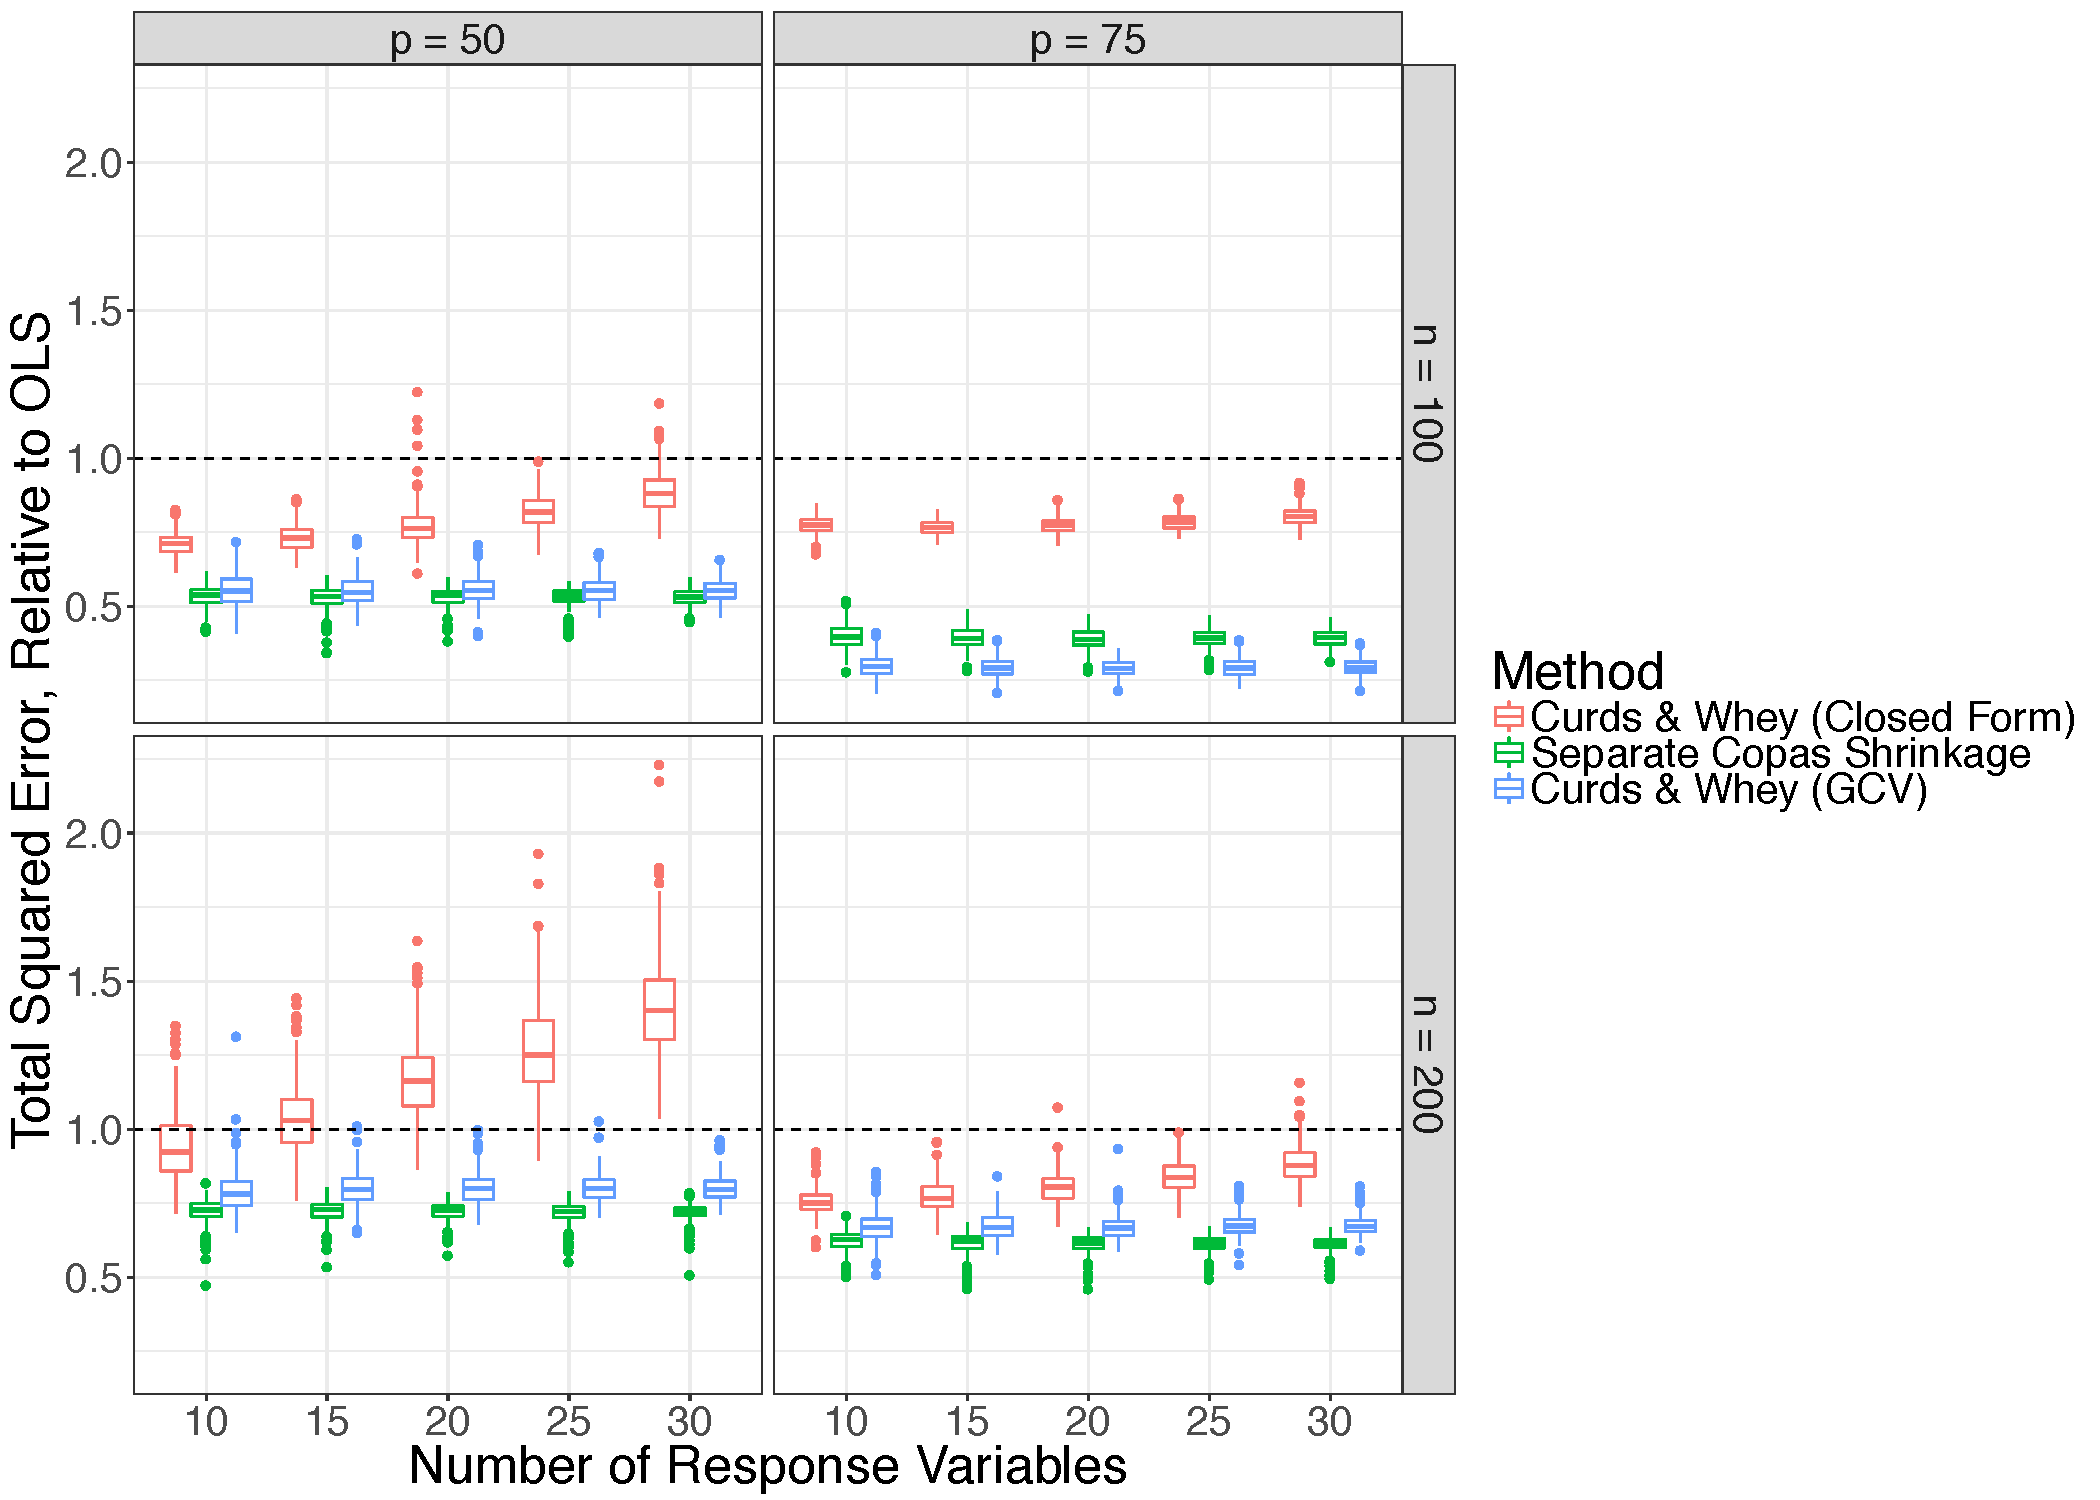
\includegraphics[width = 16cm]{../curds_n_whey/TSE_curds.pdf}
\caption{Simulation-based comparison of multi-response shrinkage methods in moderate dimensions $p$ relative to the sample size $n$. The simulation design follows Breiman \& Friedman (1997), with fixed, unit signal-to-noise ratio. The horizontal axis is the number of responses $q$ that we are modeling, and the vertical axis is the ratio $\frac{\sum_k(A_k - \widetilde{A}_k)^\T V (A_k - \widetilde{A}_k)}{\sum_k(A_k - \widehat{A}_k)^\T V (A_k - \widehat{A}_k)}$ of PTSE (modulo constants) for each method relative to OLS. Each box plot was created using $250$ runs. } %$\frac{\EE\|y-x\widetilde{A}\|_2^2}{\EE\|y-x\widehat{A}_{\text{OLS}}\|_2^2}$
\label{fig-curds}
\end{figure}



\newpage
\subsection{Extensions to Sparse Modeling}

When the number of predictors $p$ exceeds the sample size $n$, we face two major problems. First, as before, OLS is not well-defined, since $X^\T X$ is not invertible; second, CCA is also not well-defined for the same reason. Motivated by our mulitple-voxel fMRI response problem, we will assume $A$ is sparse. The first issue can be overcome by solving LASSO separately on each problem:
\begin{align}
\label{eq-separate-lasso}
\widehat{A}_{\text{lasso}}
:= \arg\min_{A'}\sum_{k=1}^q \left[\|y^{(k)} - XA'_k\|_2^2 +  \lambda_k \|A'_k\|_1\right],
\end{align}
This will be our baseline predictor, as it does not attempt to exploit any relationship between the $q$ related problems. Each $\lambda_k$ is selected via cross-validation.

\subsubsection{Subset Selection then Curds \& Whey}

One extreme is where the sparsity patterns of the $(A_k)_{k=1}^q$ are related so that the union of their support is not much larger than the largest support. Then it makes sense to replace the separable regularization term $\sum_{k=1}^q\sum_{j=1}^p \lambda_k|A_{jk}'|$ in equation \eqref{eq-separate-lasso} with $\lambda\sum_{j=1}^p \max_{k=1:q}|A_{jk}'| = \lambda\sum_{j=1}^p \|(A')^{j}\|_\infty$ to select features jointly across all of the problems. Obozinski et al (2006) relax this complete feature-sharing scenario by replacing the $\ell_\infty$ norm with $\ell_2$:
\begin{align}
\label{eq-multitask-lasso}
\widehat{A}_{\text{multitask-lasso}}
:= \arg\min_{A'}\sum_{k=1}^q\|y^{(k)} - XA'_k\|_2^2 +  \lambda\sum_{j=1}^p \|(A')^{j}\|_2.
\end{align}
This method (which can be run in \texttt{glmnet} by setting \texttt{family = "mgaussian"}) already shares strength across the different problems, but if we are using equation \eqref{eq-multitask-lasso} to select a sparse subset $\widehat{S}$ of $s$ features jointly for all $q$ problems, then we can run the Curds \& Whey procedure on $X_{\widehat{S}} \in \R^{n\times s}$ and $Y$. This requires $q+1 < s < n$, so we need to constrain $\lambda$ when doing CV. We call the resulting estimate $\widehat{A}_{\text{ML-CW}}$ for Multitask-LASSO then Curds \& Whey. This method relies heavily on feature selection, which requires a much stronger signal than getting good predictions with LASSO. The benefit is that pooling effectively affords us more observations. % grouped lasso

\subsubsection{Sparse CCA}
Given an $n\times p$ matrix $U$ and an $n\times q$ matrix $W$ with $U^\T U = I_p$ and $W^\T W = I_q$, when $n < p$ one way to make progress is to assume the canonical $u$-vectors are sparse and impose an $\ell_1$ constraint:
\begin{align}
\min_{\substack{u,w\\ \|u\|_2\lor \|w\|_2 \le 1 \\
     \|u\|_1 \le c\sqrt{p}}} u^\T U^\T W w,
\end{align}
for $c\in [0, 1]$. Note if $c = 1$ then the $\ell_1$ constraint is vacuous and this is equivalent to CCA. This assumption that the $U$-canonical directions are sparse makes sense in the context of our fMRI study, since the fMRI responses only `care' about a small number of Gabor wavelets. We use the implementation of Witten et al (2009) to obtain a $y$-canonical basis $\widehat{T}^\T$ and then pool the LASSO predictions with $\widehat{T}^{-1}\widehat{D}\widehat{T}y$ (here $\widehat{D}$ can be obtained with CV as before but can have elements bigger than $1$).

\subsubsection{Sparse Precision Estimation}
The CCA matrix $\widehat{Q} := (Y^\T Y)^{-1}Y^\T X (X^\T X)^{-1}  X^\T Y$ can be thought of as estimating $\Sigma_{yy}^{-1}\Sigma_{yx}\Theta\Sigma_{xy}$, where $\Theta = \Sigma_{xx}^{-1}$. In the simulations of Breiman \& Friedman (1997), the covariates are drawn from an $\text{AR}_p(1)$ Gaussian graphical model $(\Sigma_{xx})_{ij} = r^{|i-j|}$, which is a Markov model, and hence the inverse covariance or {\sl precision} matrix $\Theta$ is tridiagonal (by Hammersley-Clifford). If we knew of this sparse structure a-priori we could bring high-dimensional sparse precision matrix estimation to bear on constructing a plug-in estimate for $\widehat{Q}$. This seems relevant to the Gabor wavelet features of natural images, but maybe not the most direct way to take advantage of structure. \newpage

\subsubsection{Best Linear Predictor via Cross-Validation}

The goal of each of the previous extensions of the Curds \& Whey procedure was to take weighted combinations of the $q$ separate LASSO predictions $\widehat{y}$ to share strength across problems. That is, we take $\widetilde{y} = \widehat{B}\widehat{y}$ where $\widehat{B}$ is a linear predictor for $y$ based on $\widehat{y}$. Ideally, we would use the best linear predictor $B^* = \arg\min_B\EE\|y-B\widehat{y}\|_2^2$, and we can construct an unbiased estimate of this using cross-validation. The recipe is straightforward:
\begin{enumerate}
\item Split the training data into $\cv=5$ equally sized subsets. For each $v=1:5$,
\item Fit $q$ LASSO problems separately using all the data except group $v$. Let $\widehat{y}(v)$ denote the predictions on the held-out data, and $y(v)$ the true values on that subset.
\item Fit $q$ OLS problems separately. For $k=1:q$, regress $y_k(v)$ on $\widehat{y}(v)$. Write the regression coefficients in a $q\times q$ matrix $\widehat{B}(v)$. Take $\widehat{B} = \frac{1}{\cv}\sum_{v=1}^\cv \widehat{B}(v)$. 
\end{enumerate}
In small datasets, this will likely be highly variable, which can be mitigated to an extent with the choice of $\cv$. We refer to this method as Best Linear Predictor via Cross-Validation (BLP-CV).

\subsubsection{Simulations}

In Figure \ref{fig-sparse-curds} below, we compare each of these extensions to LASSO in terms of PTSE. The simulation design again follows Breiman \& Friedman (1997); specifically, we use their method for generating a block of $s$ non-zero coefficients in each problem, and then append $p-s$ zero coefficients.

\begin{figure}[h!]
\centering
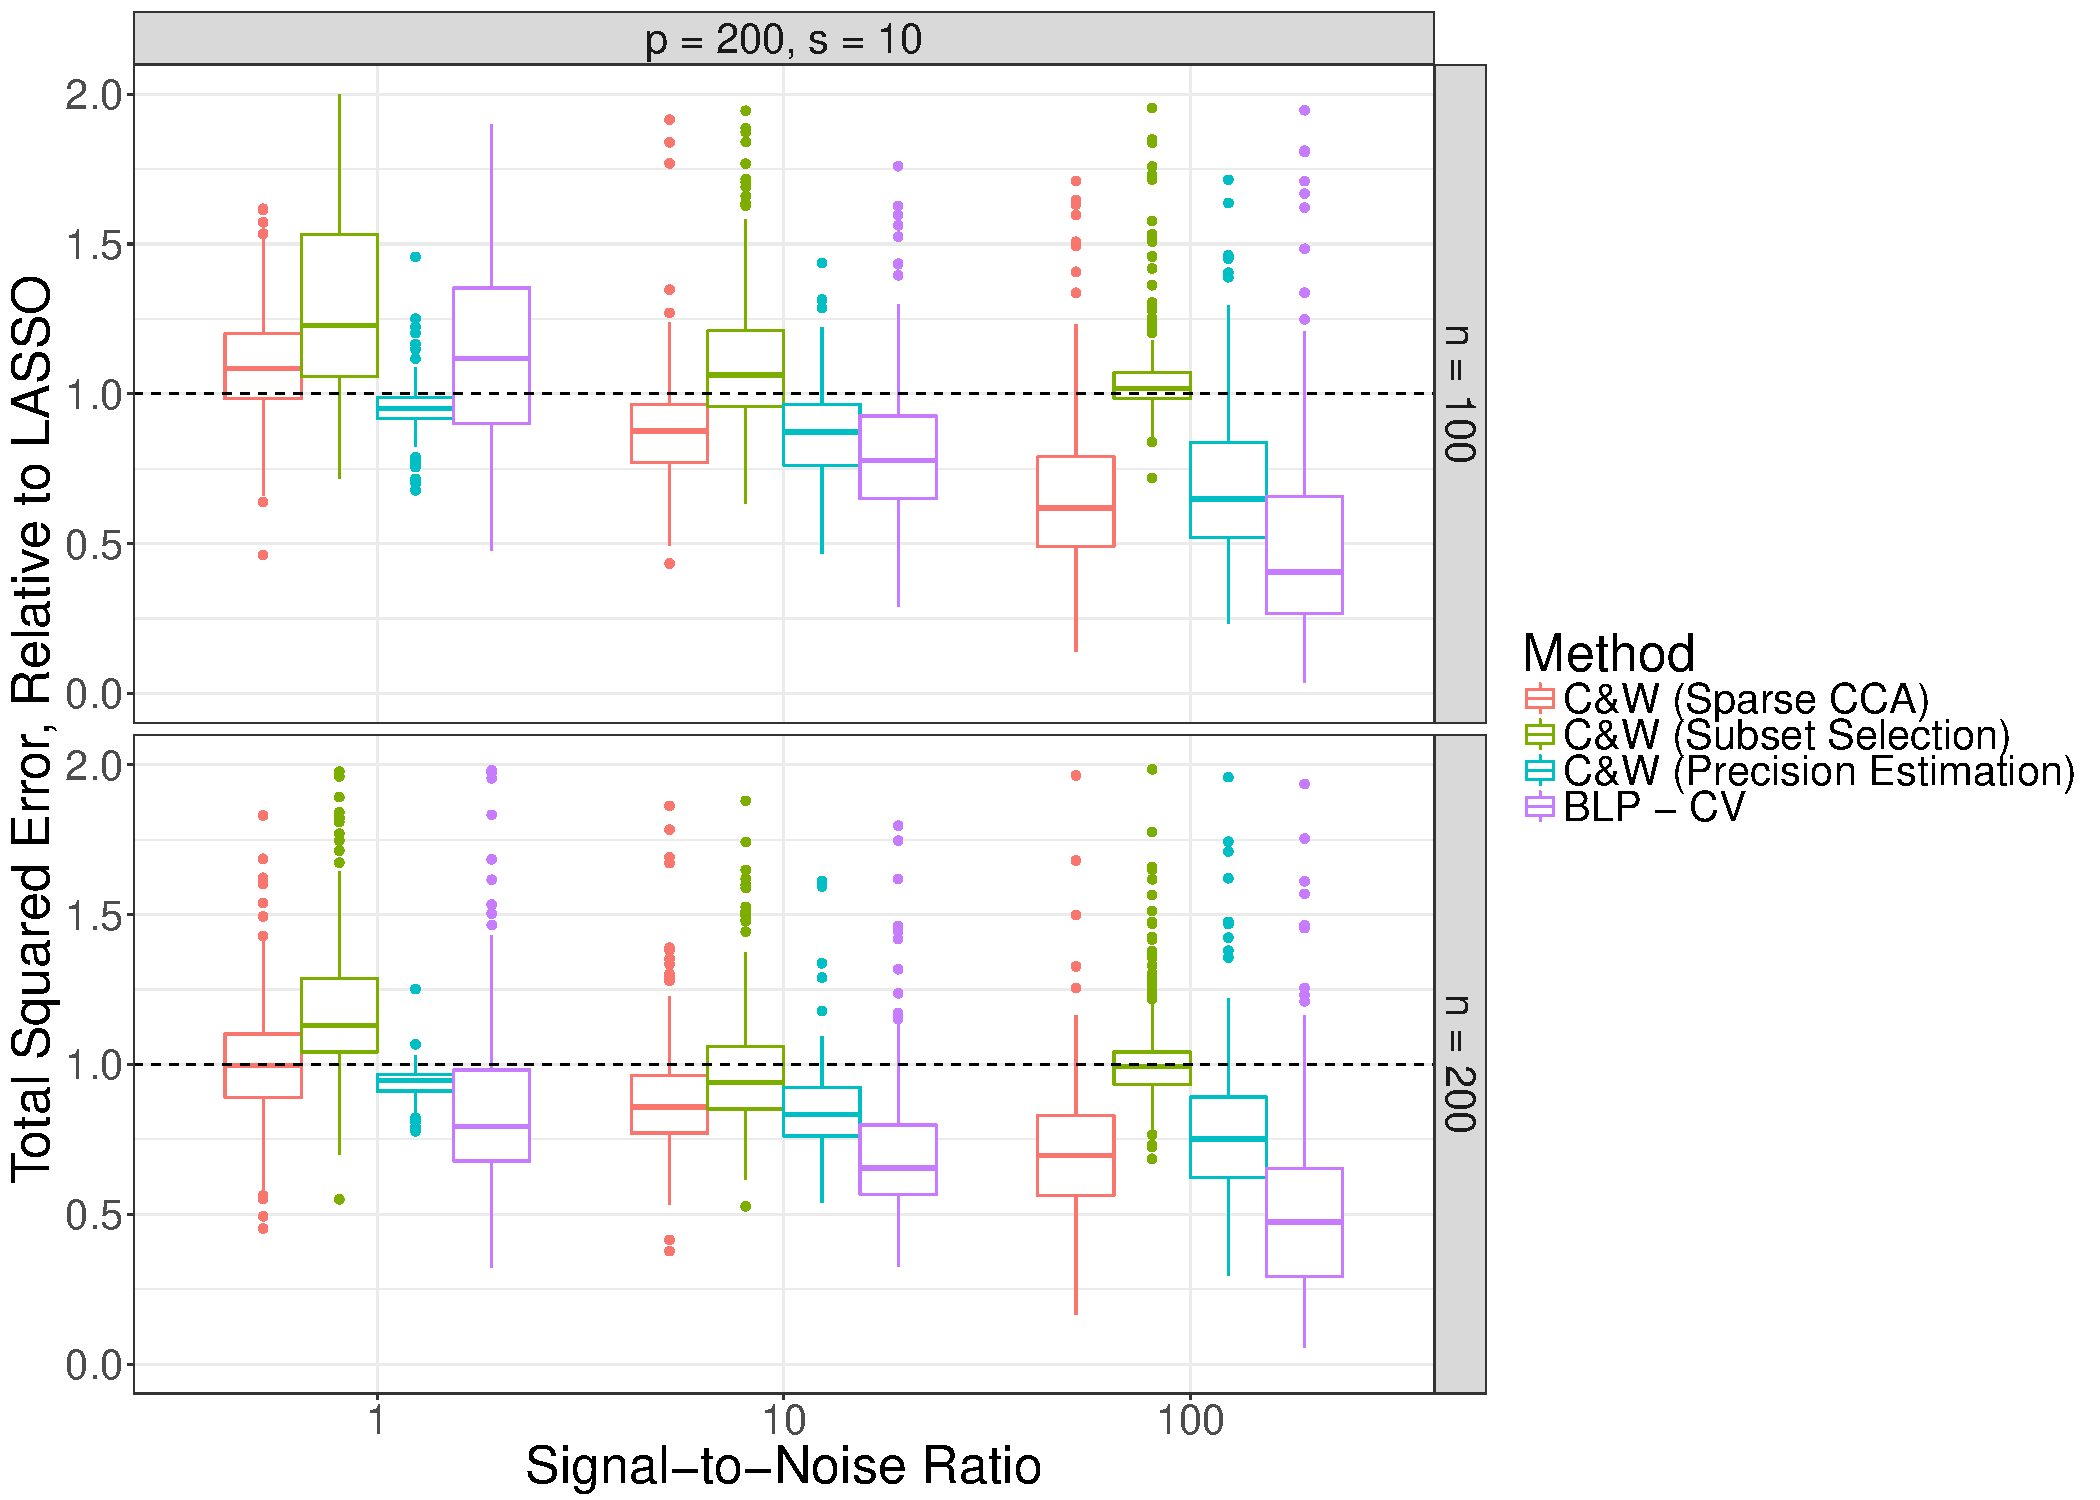
\includegraphics[width = 16cm]{../curds_n_whey/TSE_sparse_curds.pdf}
\caption{Simulation-based comparison of multi-response $(q=5)$ shrinkage methods in high dimensions $p$ relative to the sample size $n$. The setup is the same as Figure \ref{fig-curds} with additional $p-s$ zeros added. Again, each box plot was created using $250$ runs. $<1\%$ of runs went above $2$ on the vertical axis.}
\label{fig-sparse-curds}
\end{figure}

\newpage

Note since each method in Figure \ref{fig-sparse-curds} returns a $q\times p$ matrix of the form $\widehat{B}\widehat{A}_{\text{lasso}}$, each is strictly slower to compute than LASSO, but the computational cost of estimating $\widehat{B}$ also varies. The Sparse Precision Estimation method is by far the fastest, since it assumes the model $(\Sigma_{xx})_{ij} = r^{|i-j|}$, estimates $r$ via autocorrelation, and then computes the tri-diagonal inverse in closed form. Since this model is correct in our simulations, this yields a fairly reliable plugin estimate of the CCA matrix, even in high dimensions.

The next fastest method is running Curds \& Whey on a subset of the covariates. This in part because, rather than running \eqref{eq-multitask-lasso}, we estimate the support directly from $\widehat{A}_{\text{lasso}}$. As implemented, subset selection does not do consistently better than LASSO, even when the SNR is {\bf obscenely high}. This is surprising in light of Figure \ref{fig-curds}, since if we knew the support exactly, this method would even beat OLS run on the support (which definitely beats LASSO in prediction error). This result appears to underscore the difficulties of subset selection.

The matrix algebra in computing the ordinary CCA matrix ($q<p<n$) should be $\co(qp^2)$. The cost of this implementation of sparse CCA is unclear. The algorithm runs for a fixed number of iterations ($15$), and each update has a single matrix-vector product $\co(qs)$ where $s\ll p$ is the sparsity level as well as a grid search. In terms of wall-clock time, the Sparse CCA approach is the third fastest. As in the GCV approach to Curds \& Whey, we run Sparse CCA $\cv + 1 = 6$ times, and that's the bulk of the computational cost.

The BLP-CV approach is a clear front-runner in terms of relative improvement over LASSO but also computational cost. The algorithm takes roughly $\cv+1 = 6$ times as long to run as LASSO. In the top left of Figure \ref{fig-sparse-curds} (relatively low signal and sample size), LASSO beats BLP-CV most of the time, so it's not always true that the added computational cost will be worth it.

\subsection{Application to fMRI Study}

A single subject observed a total of $n = 1750$ images, each of shape 128 $\times$ 128. After pre-processing each image using a Gabor wavelet pyramid, $p = 10921$ covariates remain, and we observe the fMRI response in $q=20$ voxels. In Figure \ref{fig-features} we display two intermediate layers of the Gabor wavelet pyramid. Most (over $8000$) of the features are on the finest level of the pyramid, which are localized to patches a few pixels wide.

\begin{figure}[h!]
\centering
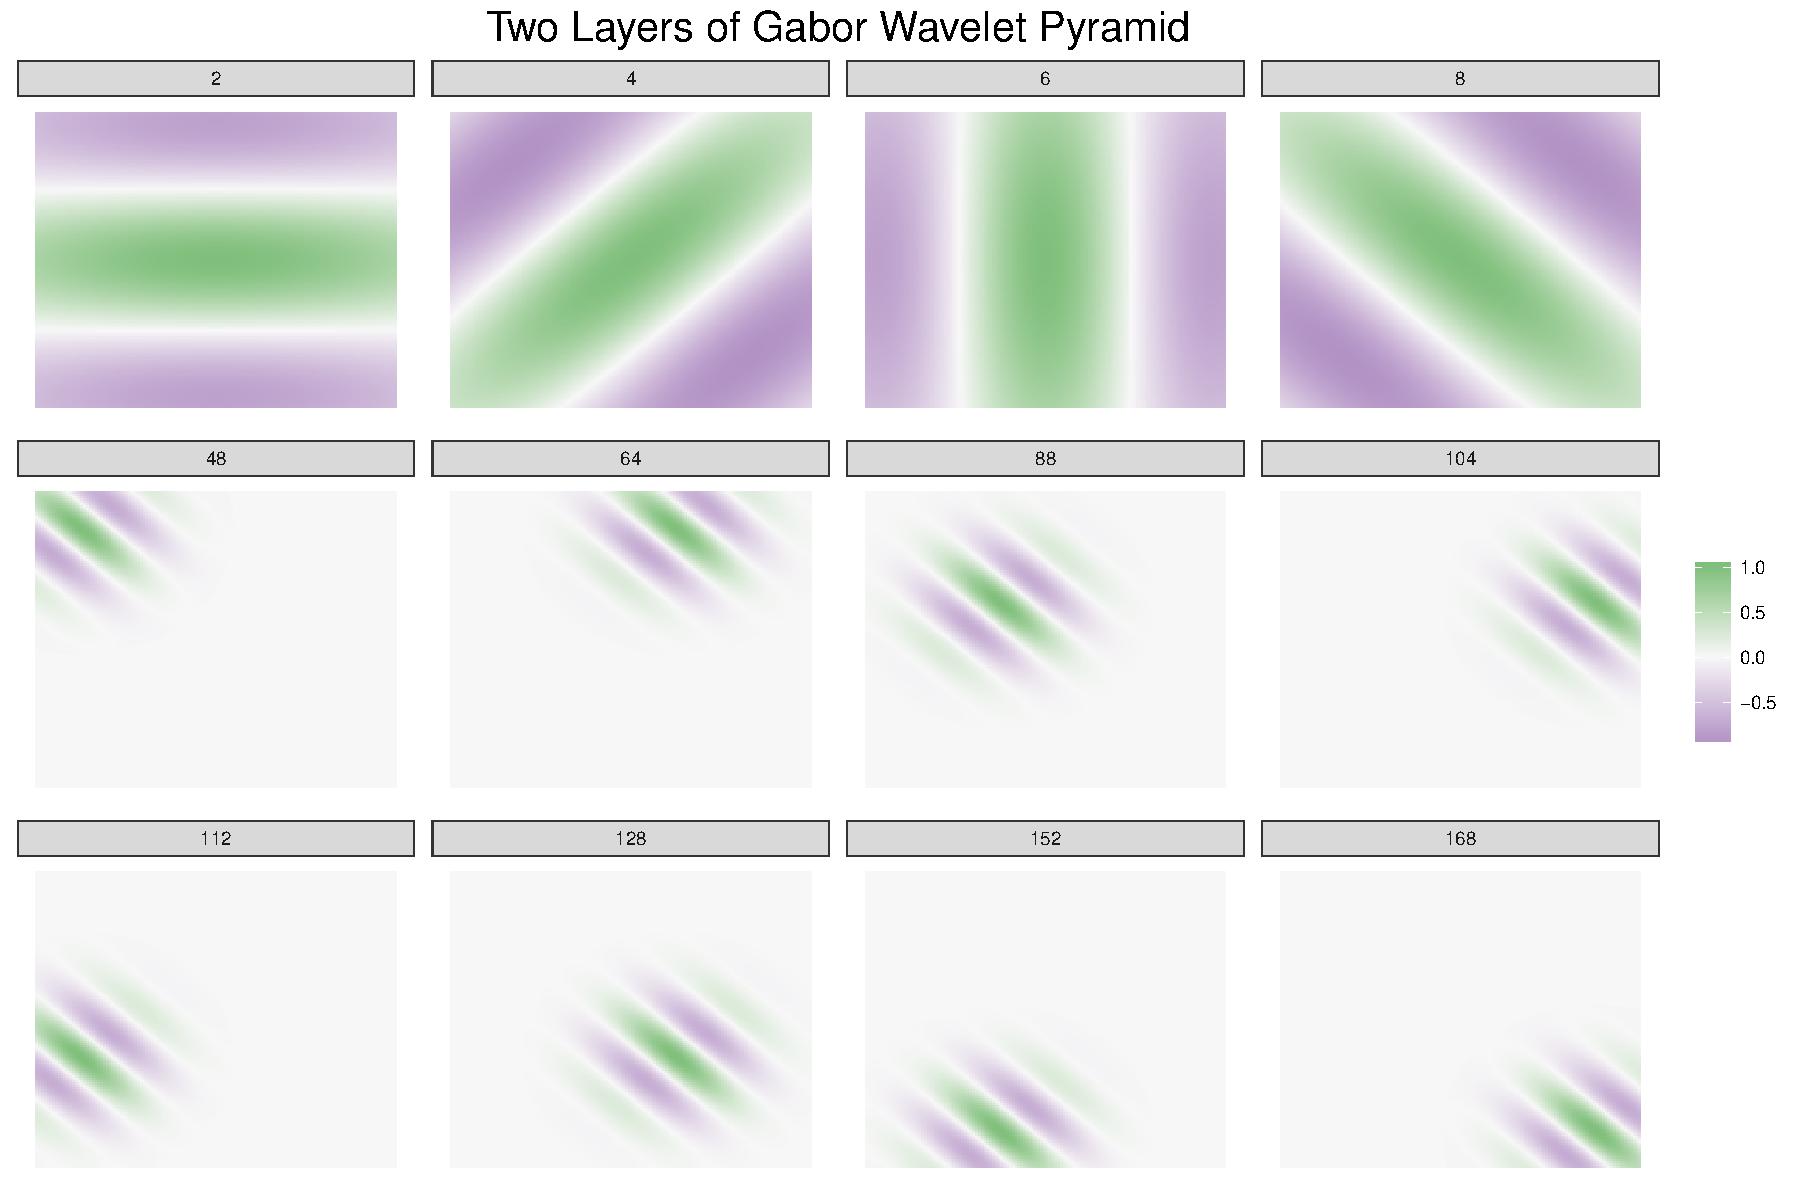
\includegraphics[width = 12cm]{../fmri_study/plots/wav_viz.pdf}
\caption{Understanding the features by the transforms they represent. Each feature is a coefficient from the image convolved with a wavelet basis element. Up in the pyramid, the wavelets depend on the entire 128 $\times$ 128 image; toward the bottom wavelets are localized to a small patch.}
\label{fig-features}
\end{figure}


\newpage

\noindent In Figure \ref{fig-cor} below we note that the fMRI responses for different voxels are indeed (positively) correlated, with one block of voxels having much stronger correlations than the others. 

\begin{figure}[h!]
\centering
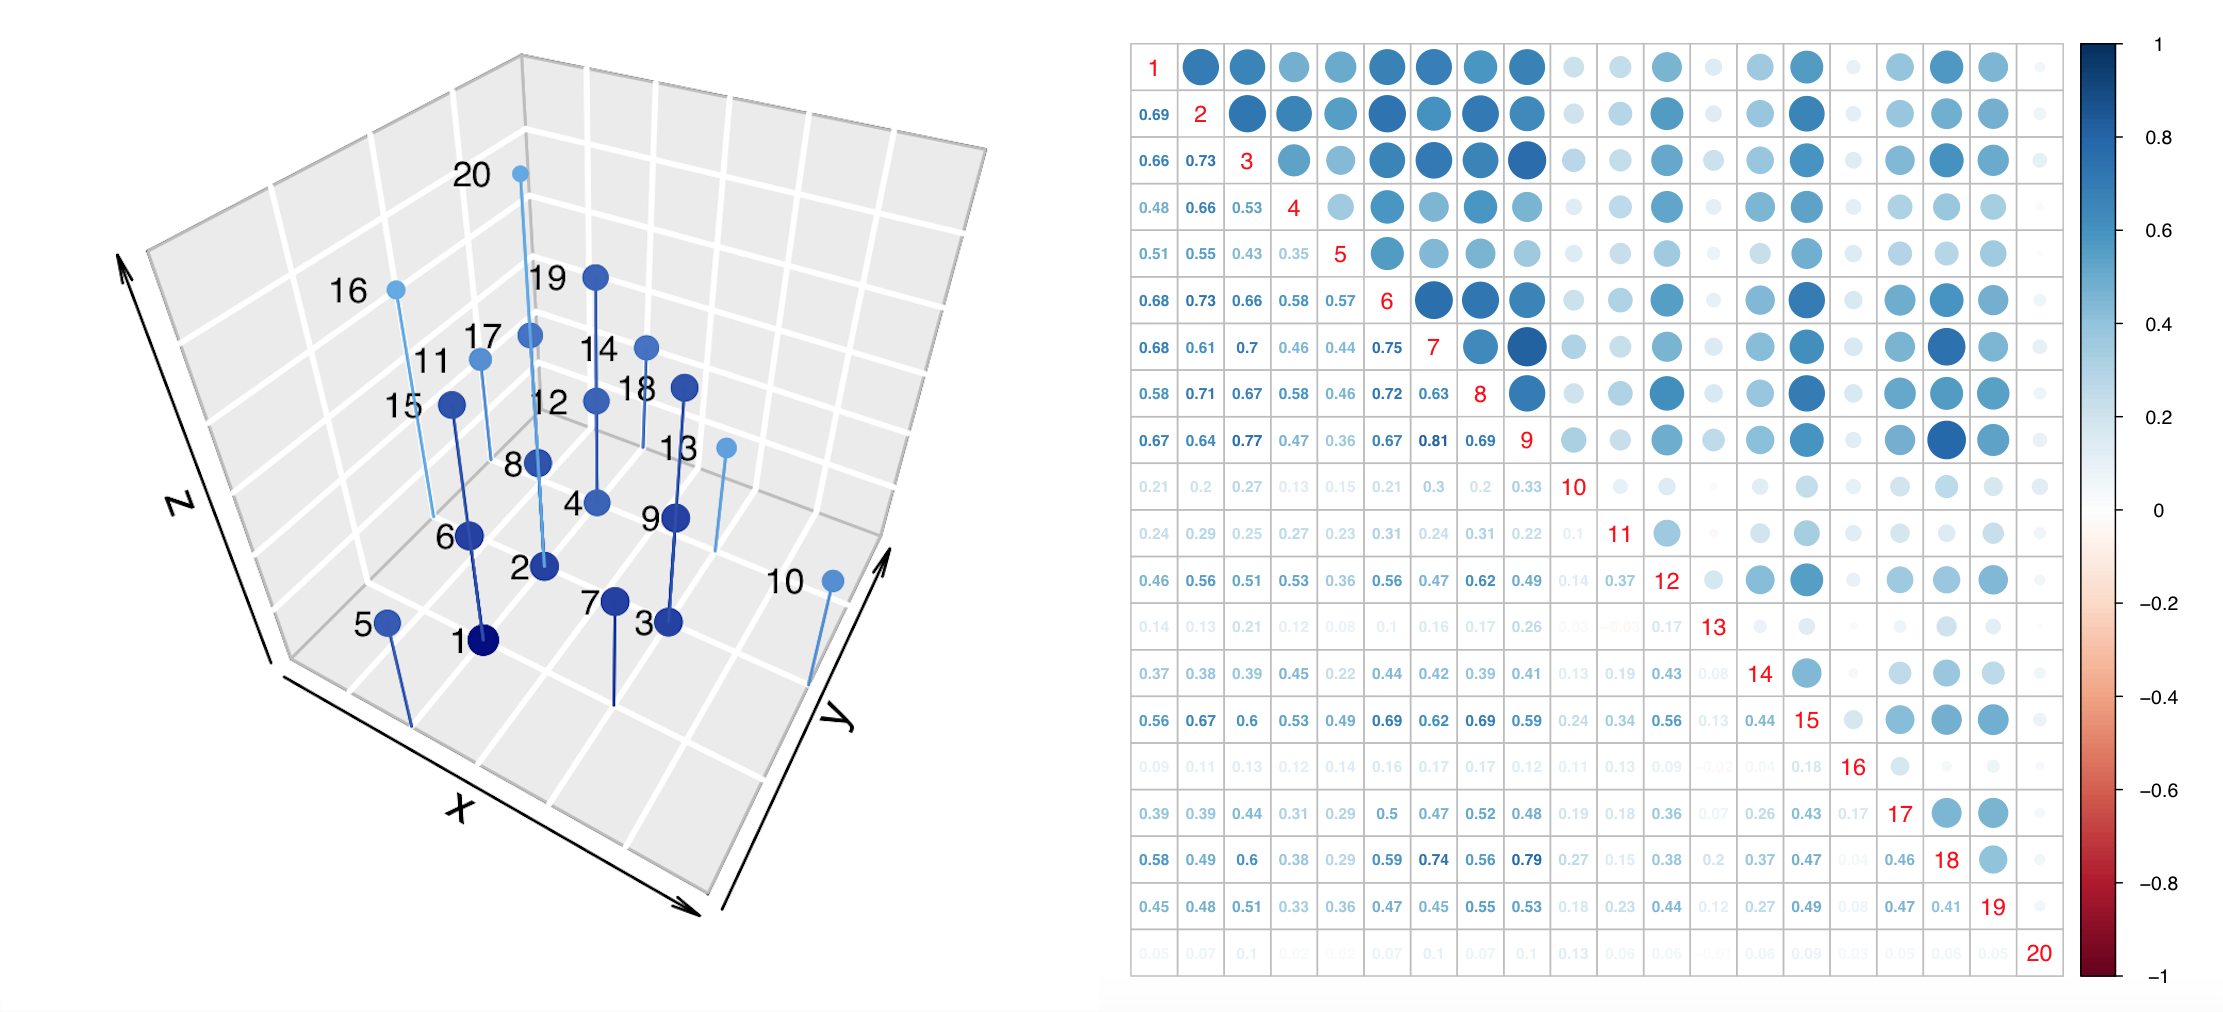
\includegraphics[width = 14cm]{../fmri_study/plots/corr_plot}
\caption{Left: Each voxel in relative spatial coordinates, colored (and sized) proportional to the correlation between that voxel's fMRI responses and those of voxel 1. Right: pairwise correlations between voxels. The first row of this thus gives the intensities for the 3D-plot on the left.}
\label{fig-cor}
\end{figure}

In keeping with Kay et al (2008) who published this data, we use the correlation between the predicted responses $\widehat{y}$  and the observed responses $y$ on test set to measure the performance of our models. In Figure \ref{fig-cor}, we find that estimating the matrix $\widehat{B}$ via cross validation does not appear to help much by this measure.

\begin{figure}[h!]
\centering
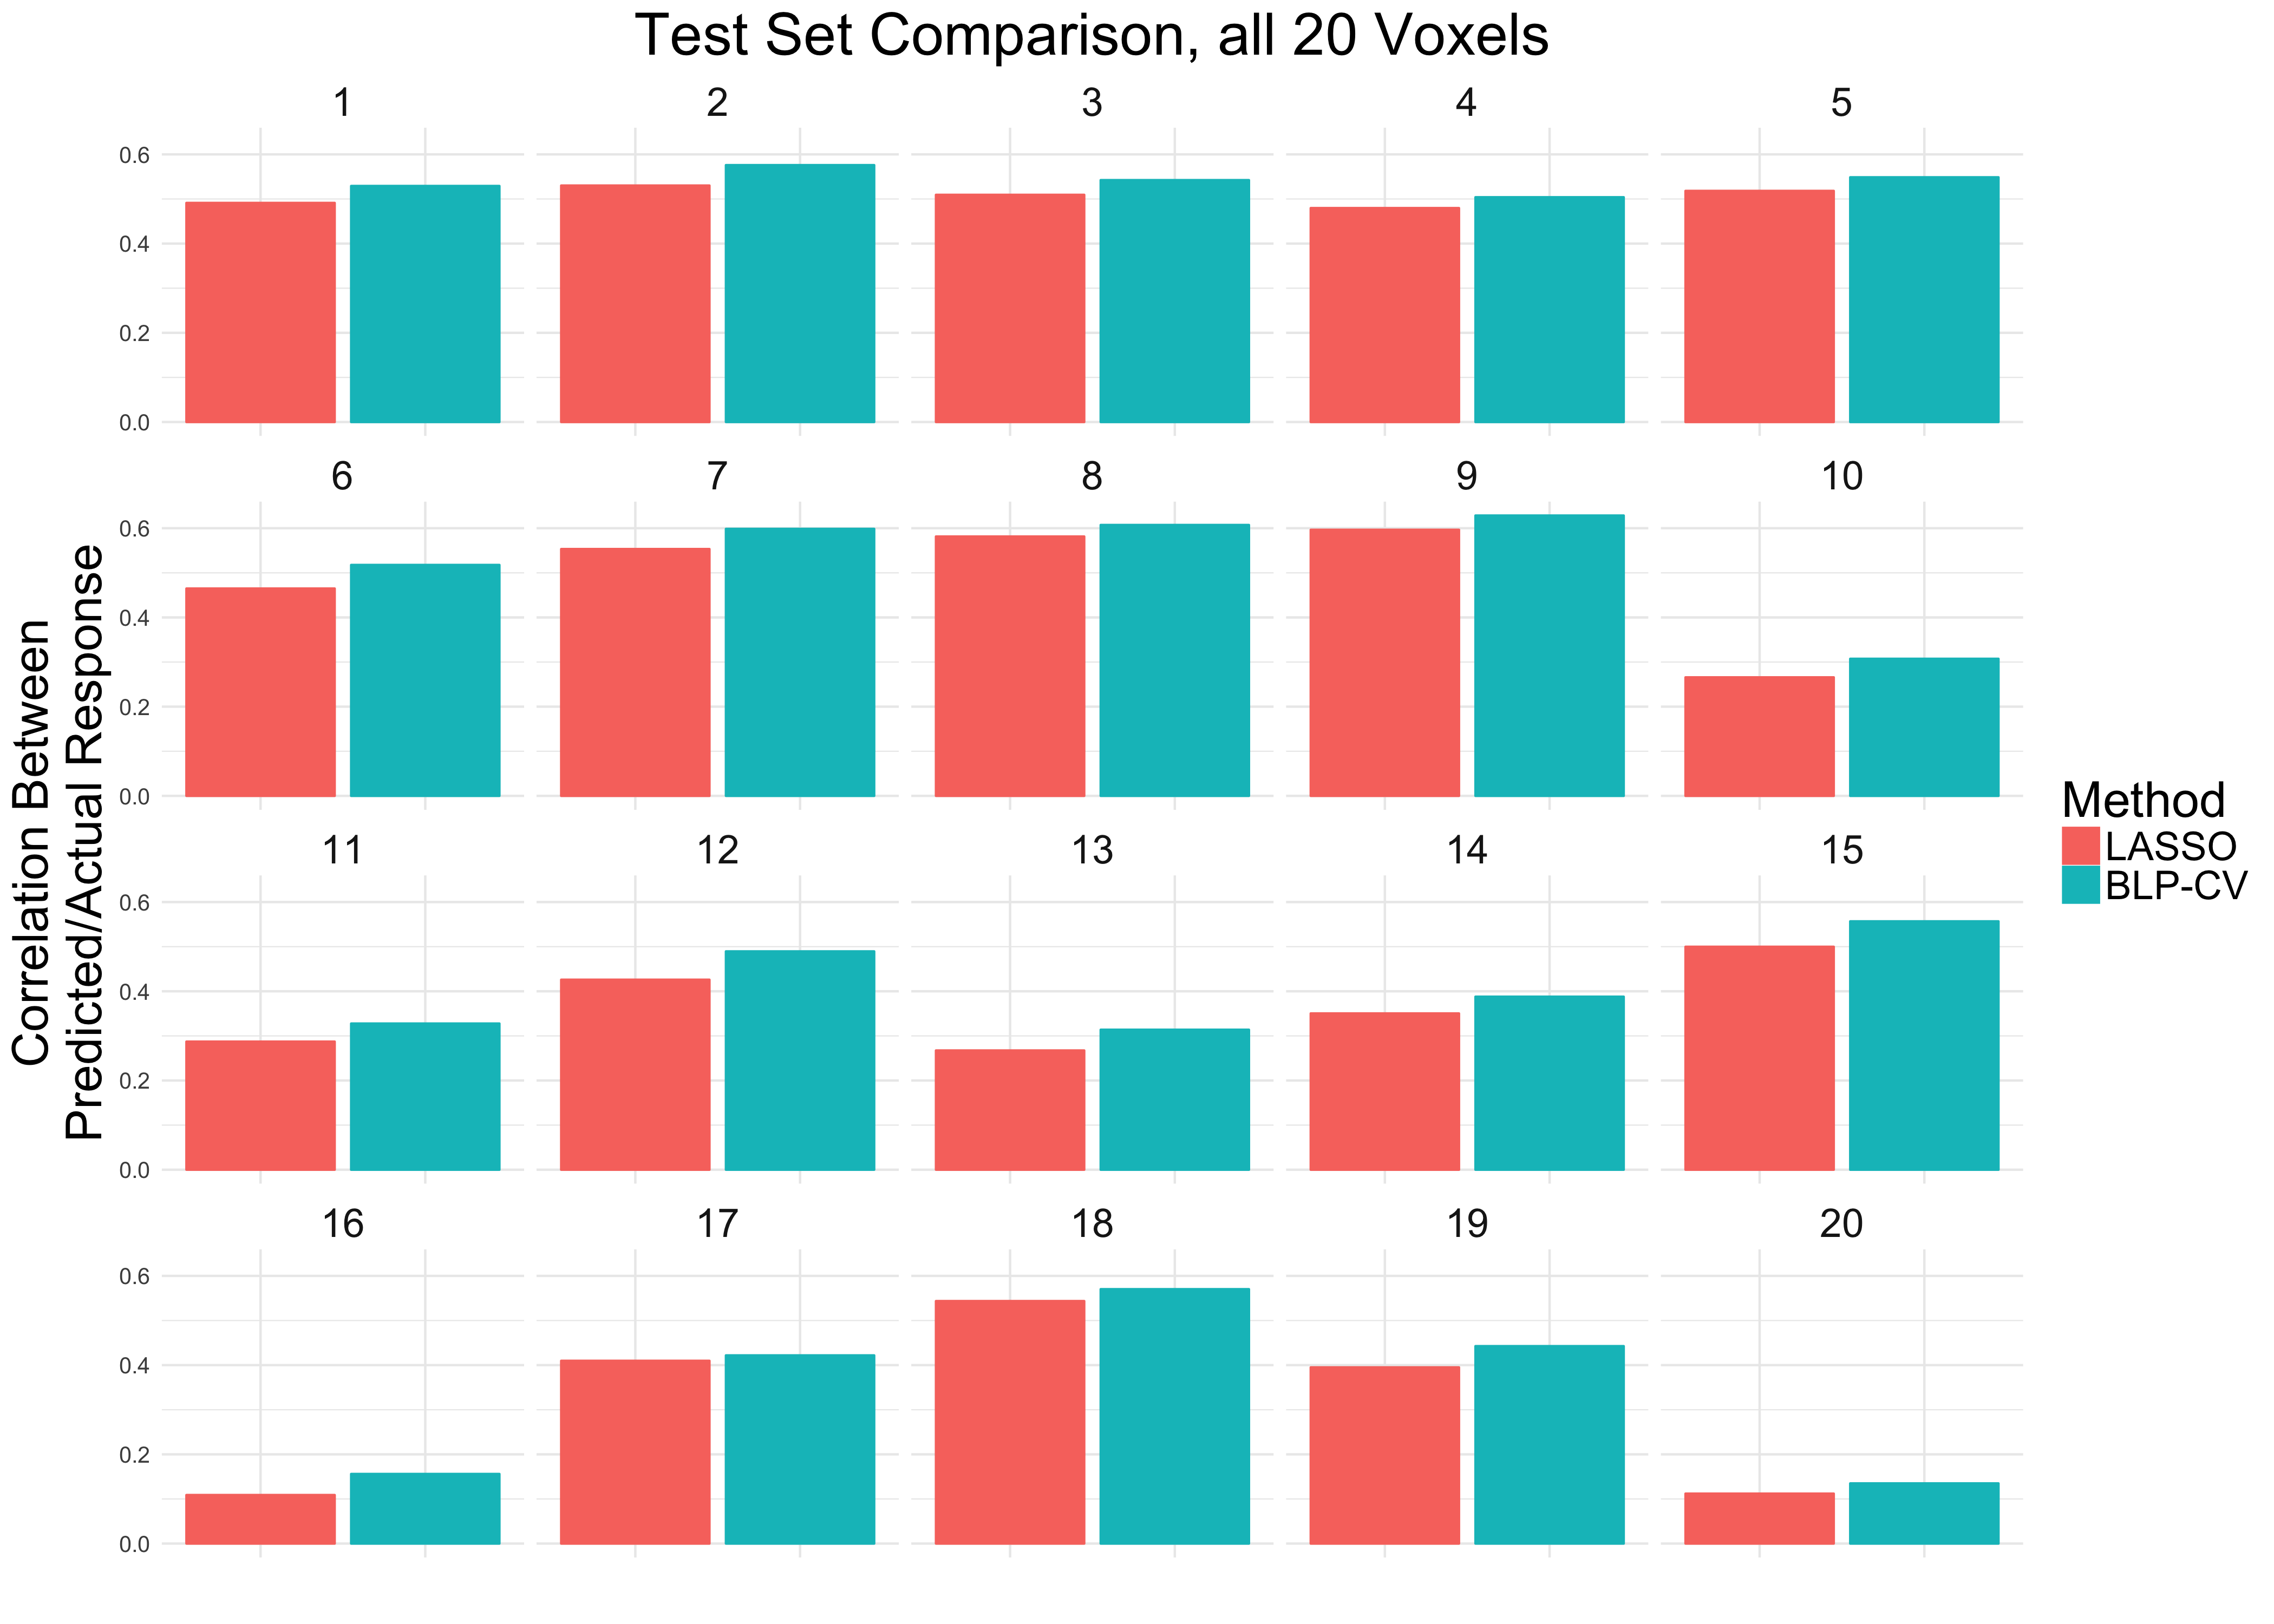
\includegraphics[width = 14cm]{../fmri_study/plots/cors.png}
\caption{Model comparison using the test set. We report the correlation between fitted and observed fMRI response values for all voxels.}
\label{fig-cor}
\end{figure}

\end{document}
